\documentclass{uflamon-22}          % classe base para a monografia


%==============================================================================
% Utilizacao de pacotes
\usepackage[utf8]{inputenc}
\usepackage[T1]{fontenc}         % usa fontes postscript com acentos
%\usepackage{times}              % usa fonte times como default
\usepackage[brazil]{babel}       % hifenização e títulos em português do

\usepackage{amsmath}             % pacote da AMS para Matemática Avançada
\usepackage{amssymb}             % símbolos extras da AMS
\usepackage{latexsym}            % símbolos extras do LaTeX
\usepackage{graphicx}            % para inserção de gráficos
\usepackage{listings}            % para inserção de código
\usepackage{fancyvrb}            % para inserção de saídas de comandos
\usepackage{multirow}
\usepackage{caption2}

\usepackage[ruled,lined]{algorithm2e}
\usepackage{algorithmic}

\usepackage{colortbl} % frescuras em tabelas
\newcolumntype{L}{|>{\columncolor[gray]{0.9}}l|} %multicolunas boiolas

% cores para os links cruzados
\usepackage{color}
\definecolor{rltred}{rgb}{0.0,0,0}
\definecolor{rltgreen}{rgb}{0,0.0,0}
\definecolor{rltblue}{rgb}{0,0,0.0}

\usepackage[colorlinks=true,
	        urlcolor=rltblue,       % \href{...}{...} external (URL)
   	     filecolor=rltgreen,     % \href{...} local file
      	  linkcolor=rltred,       % \ref{...} and \pageref{...}
     		  citecolor=rltgreen,
    		  pdftitle={Dissertacao_Luiz_Costa},
			  pdfauthor={Luiz_costa},
           pdfsubject={},
           pdfkeywords={}%
]{hyperref} % para referência cruzadas
%\usepackage{hyperref}            % para referência cruzadas
%\usepackage{subfigure}           % figuras dentro de figuras




            % remodelando o formato dos títulos de 
                                 % tabelas e figuras

% % configuração padrão do listings   
 \lstset{
    language=Java,
    extendedchars=true,
    tabsize=3,
    basicstyle=\footnotesize\ttfamily,
    stringstyle=\em,
    showstringspaces=false 
 }

\titleformat{\paragraph}
{\normalfont\normalsize\bfseries}{\theparagraph}{1em}{}
\titlespacing*{\paragraph}
{0pt}{3.25ex plus 1ex minus .2ex}{1.5ex plus .2ex}

\usepackage[alf,abnt-etal-cite=3,abnt-etal-list=0,abnt-etal-text=emph, bibjustif]{abntcite}


% redefinindo formatação de títulos de tabelas e figuras
\renewcommand{\captionfont}{\small}
\renewcommand{\captionlabelfont}{\small \bfseries}

% para referências de acordo com a ABNT
% precisa instalar o abntex antes!!!
% http://abntex.codigolivre.org.br/
% comente se pretende usar outro padrão
%\

%==============================================================================
% para os fãs do Word, descomente as linhas abaixo
%\sloppy 
%\usepackage{identfirst} 



%==============================================================================
% definido comandos na monografia - não é necessário na sua monografia 
% apenas para exemplificar a definição de novos comandos



% Especificando hifenizações que por ventura LaTeX não saiba fazer
% Por padrão 99,9% dos termos em português devem ser hifenizados corretamente.
\hyphenation{}

%==============================================================================
% Dados da monografia, capa: autor, titulo, banca, etc... - SUBSTITUA DE ACORDO
%==============================================================================
\author{Luiz Augusto Guimarães Costa}
\title{Análise da utilização de agente de software sobre Redes Veiculares Hibridas.}
\date{2013}
\tipo{Dissertação apresentada à Universidade Federal de Lavras,como parte das exigências do Programa de Pós-Graduação em Ciência da Computação, área de concentração em Ciência da Computação, para obtenção do título de Mestre}
\areaconcentracao{Transporte de agentes;Comunicação Oportunistas; Agentes de Software; Redes Ad Hoc, VANET; MANET}
\orientador{Wilian Soares Lacerda}
%\coorientador{Tales Heimfarth} 
%\coorientadordois{Prof. Tiag�o Meganha} % comente se n�o tiver coorientador
\bancaum{}
%\bancauminst{}
%\bancadois{Wilian Soares Lacerda}
%\bancadoisinst{}
%\bancadois{Prof. Beltrano Tomazio Fiuxcrute} % comente se sua banca tiver s� um
%professor
%\bancatres{Fulanim de Sicrano}% comente se sua banca tiver só um professor
\defesa{}
\palchaves{Transporte de agentes;Comunicação Oportunistas; Agentes de Software; Redes Ad Hoc, VANET; MANET}
\keywords{Agent Ferrying; Opportunistic Communication; Software Agents; Ad Hoc Networks; VANET; MANET}
%==============================================================================

%% dados para ficha catalográfica
% primeiro autor
%\fcautor{Costa, Luiz Augusto Guimarães}
% autores, separados por vírgula
%\fcautores{Luiz Augusto Guimarães Costa, Tales Heimfarth}
% dados para ficha catalográfica conforme modelo da BC-UFLA 
%\fccatalogacao{ }
% classificação de acordo com a CDD, comente se não tiver isso.
%\fcclasi{003.5}
%\fcclasii{005.43}
%\scalenumwidth{1.5} % Aumenta espaco do numero das secoes no sumario em escala
% Aqui comeca o documento propriamente dito


\begin{document}

\maketitle

%\pagestyle{empty}

%\dedic{}

%\thanks{}

%\resumo{resumo em português}

%\resumoingles{resumo em inglês}

\listoffigures
\listoftables
\tableofcontents

\pagestyle{ufla}

%\section{Introdução}

Comunicação sem fio permite novas aplicações que exploram a transferência de dados entre nós móveis. Redes oportunistas são redes onde a comunicação não é continua, isto é, nunca deve existir um caminho pré-definido entre o nó de origem e o nó destino. Isto proporciona suporte para os cenários em que os dados são transportados a partir de uma fonte para um destino através dos nós móveis que levam fisicamente os dados de um lugar para outro, com ou sem auxilio de uma infraestrutura fixa. Essas características podem ocorrer em uma série de aplicações tolerantes ao atraso \cite{Fall:2003}. Entretanto, esse paradigma exige um maior número de nós para auxiliar o transporte dos dados, assim melhorando a probabilidade deles serem eventualmente entregues. Neste ponto, a utilização dos nós mais promissores para transportar os dados proporcionam uma maior probabilidade desses dados alcançarem o seu destino \cite{Freitas:2013}.

O uso de dispositivos móveis na formação de uma rede \emph{ad hoc} abriu um novo horizonte para exploração de técnicas de comunicação oportunísticas. Um exemplo de comunicação oportunística acontece quando dados são transportados por nós móveis de uma origem para um destino utilizando-se a movimentação física do nó. As conexões temporárias entre nós que estão próximos geograficamente durante um pequeno intervalo de tempo, são explorados sem a existência de uma rede conectada constantemente. Esse tipo de comunicação exige da aplicação tolerância a atrasos consideráveis e desconexões frequentes. Muitos cenários reais podem fazer uso dessa abordagem.

Sistemas que exploram esse tipo de comunicação exigem a existência de um grande número de nós, de forma a aumentar a probabilidade de sucesso na entrega dos dados. Outra questão importante neste tipo de rede é a utilização de informações baseada no contexto que permitem uma decisão eficiente para transporte de dados entre os nós. 

O uso de agentes móveis representa uma tecnologia promissora \cite{Urra:2010} para tratar os problemas aqui apresentados. O seu uso permite o encapsulamento de inteligência na rede, melhorando as decisões que serão responsáveis pelo trafego de dados \cite{Freitas:2010}. Essa abordagem oferece flexibilidade para elaborar estratégias de transporte dos dados, assim permitindo enfrentar possíveis problemas encontrados de forma mais ágil. 

O transporte de agente utiliza o mesmo principio de transporte de dados, mas em vez de apenas dados, um agente também transfere o seu comportamento. A vantagem de usar agentes para transportar dados é que eles não são limitados a um protocolo de roteamento instalados nos nós, mas como parte de sua própria inteligência, eles podem fornecer a sua própria estratégia para mover através dos nós na rede. Isto é a responsabilidade da decisão do dado migrar ou não de um nó para outro é delegada ao agente, assim aumentando a capacidade de contornar as adversidades proporcionadas por ambientes instáveis.

Com essa abordagens as redes veiculares deixam de ser construídas para uma determinada finalidade, deixando para o software do agente definir a finalidade. Assim a mesma rede onde existe um ciclista com equipamentos que permitem o envio de agentes que avisam os veículos de sua presença pode ser utilizada por um hotel que oferece quartos para motoristas cansados. 

A versatilidade do agente aumenta se os veículos possuírem sensores que possam captar a situação do condutor do veículo, por exemplo se ele esta embriagado avisar a policia. Outra aplicação é em caso de acidente o próprio veículo cria agentes que avisam os veículos vizinhos, cria outro agente para buscar um veículo da policia nas proximidades e outro para buscar uma ambulância mais próximos.   

\subsection{Objetivo}

O objetivo principal desse projeto é a exploração de agentes de software para encaminhar dados utilizando informação geográficos sobre uma VANET. Pretende-se estudar o impacto da utilização da infraestrutura fixa sobre o agente de software.

Como um segundo objetivo é avaliar o padrão ZigBee quanto aos requisitos necessários para a criação de uma VANET capaz de transportar agentes. 

Serão propostos duas redes veiculares \emph{ad hoc} (VANET), uma rede híbrida e outra somente com veículos. Os agente serão desenvolvidos no ambiente de simulação GRUBIX, desenvolvido pelo Grupo de Redes Ubíquas do Departamento de Ciência da Computação da Universidade Federal de Lavras, baseado no simulador Shox \cite{Lessmann:2008}.

Para realizar a avaliação dos agentes serão desenvolvidos dois cenários. O primeiro uma rede somente com veículos e o segundo uma rede híbrida. Ambos os cenários serão examinados em uma cidade com quadras do mesmo tamanho, essa cidade é baseada no modelo de movimento \emph{Manhattan} \cite{Bai:2003}. O desenvolvimento dos dois cenários servirá para análise do desempenho dos agentes em ambientes diferentes e com distribuição dos veículos. Cada veículo presente nos cenários dispõe de um dispositivo de comunicação sem fio e um GPS (\emph{Global Positioning System}) que serviram de infraestrutura para o agente. 

Após a realização das simulações será desenvolvido um equipamento capaz de hospedar o agente. Também esse equipamento será avaliado nos dois cenários simulados.  

\subsection{Motivação}

Segundo a \cite{oms:2013}, 1,24 milhões de pessoas morreram no trânsito em todo mundo em 2010. Um estudo \cite{Cintra:2012} aponta que o trânsito caótico da cidade de São Paulo impõe um prejuízo de R\$ 50 bilhões por ano ao Brasil. A redes sem fio \emph{ad hoc} proporcionam um novo horizonte para a melhoria das condições do trânsito em grandes metrópoles. Essas redes podem recolher dados em tempo real sobre o trânsito, assim proporcionando aos condutores e autoridades informações importantes para favorecer a segurança no trânsito.  	

Entre várias aplicações possíveis em VANET, as que proveem maior segurança do trânsito são as que recebem maior atenção. Alguns situações de riscos poderiam ser evitados caso os motoristas tivessem informações de eventos ou situações do trânsito em tempo real.

Na literatura existem poucos trabalho práticos em VANET se comparado com os trabalhos envolvendo simulações. Isto acontece por que existem poucos equipamentos e o custo deles são elevados. Atualmente existe um padrão de redes veiculares IEEE 802.11p \cite{Jiang:2008}. O padrão 802.11p pode ser atualizado assim que as pesquisas avançarem. Então o ZigBee pode ser uma nova direção para o desenvolvimento dessas redes \cite{Bhargav:2013}. 

As redes veiculares é um tópico em constantes pesquisa pelo setor público e privado. Sua grande flexibilidade e suporte a várias aplicações para melhorar a qualidade de vida nos grandes centros urbanos foram atributos que motivaram o desenvolvimento deste trabalho.

\subsection{Estruturado Trabalho}

Este trabalho está organizado da seguinte forma: os conceitos sobre redes veiculares, agentes de software e modelos de movimentos são apresentados na Seção \ref{sec:referencialTeorico}. Os procedimentos para a realização das simulações e a especificação para a construção do protótipo são apresentados na Seção \ref{sec:metodologia}. Na Seção \ref{sec:resultados} os resultados são apresentados e discutidos. Enfim, a conclusão do trabalho e proposta de continuidade são apresentados na Seção \ref{sec:conclusao}.

%\section{Referencial Teórico}
\label{sec:referencialTeorico}

O presente capítulo apresenta os conhecimentos necessários para a compreensão dos assuntos relacionados ao trabalho. 

\subsection{Redes \emph{Ad Hoc}}

Uma rede \emph{ad hoc} é definida como uma coleção de entidades móveis interligados por uma tecnologia sem fio, formando uma rede temporária sem a ajuda de qualquer administração ou qualquer tipo de apoio fixo \cite{Zafoune:2007}. É um tipo descentralizado de rede, visto que não depende de uma infra-estrutura pré-existente, como roteadores em redes com fio ou pontos de acesso em redes sem fio \cite{Niazi:2009}. Outra característica é a capacidade das redes \emph{ad hoc} adequarem a condição da conectividade da rede, distribuindo a responsabilidade de organização e controle da rede para os nós, podendo determinar se um nó vai transmitir ou não dinamicamente \cite{Rezende:2008}.

As redes \emph{ad hoc} possuem características próprias que a tornam adequadas a situações onde não existe uma infra-estrutura de comunicação presente \cite{Niculescu:2003}. Elas também podem ser utilizadas em situações onde não seja possível utilizar nós críticos para organização ou controle da rede, pois o desempenho da rede \emph{ad roc} não é afetado se um nó falhar ou mesmo sair da rede \cite{Dressler:2008}.

\subsection{Redes Tolerantes a Interrupção}
Segundo \cite{Nichols:2007}, \emph{Delay-tolerant networking} (DTN) são redes projetadas para trabalhar em ambientes com comunicação instável ou temporária produzido por limitações ou anomalias, causando o menor impacto negativo possível na aplicação. 

O autor \cite{Burgess:2006} sugere que rotas instáveis podem ser causadas por problemas como: a alta mobilidade dos nós, a baixa densidade de nós, uma curta faixa para transmissão de dados ou interferências ambientais.

A DTN é uma arquitetura de rede muito utilizada atualmente na exploração do espaço ou de planetas distantes \cite{Spyropoulos:2010}, por que o espaço é um ambiente hostil que proporciona um longo período de latência no sinal, como também existe uma grande interferência eletromagnética.

 \subsection{Redes Moveis \emph{Ad Hoc}}
A \emph{Mobile Ad Hoc Networks} (MANET) é uma categoria de redes \emph{ad hoc} \cite{Rezende:2008} onde os nós são livres para deslocarem enquanto se comunicam com outros nós. Por causa da natureza dinâmica da MANET os dados que trafegam por ela podem ser corrompidos ou perdidos com facilidade \cite{Bai:2003}.

Essa configuração de rede proporciona uma frequente perda de conexão entre os nós, portanto as MANETs precisam de protocolos que possam estabelecer uma boa qualidade de serviço \cite{Bai:2003}. Essas características móveis permitem que grupos de celulares possam se conectar sem precisar de uma infraestrutura fixa somente criando uma rede \emph{ad hoc} \cite{Piorkowski:2009}.

 \subsection{Redes Veiculares Ad Hoc}



As \emph{Veicular Ad Hoc Networks} (VANET) são um conjunto de veículos que possuem capacidade computacional e estão ligados em uma rede. A VANET é um tipo de MANET que não possuem recursos limitados, então não existe a necessidade de preocupação com uso de recursos como por exemplo energia, processamento e memória \cite{Loulloudes:2010}.

A velocidade dos nós é outro fator importante no desenvolvimento de uma VANET \cite{Kumar:2011}, partindo do princípio que veículos possuem uma velocidade muito maior de deslocamento do que dispositivos móveis. 

O autor \cite{Kumar:2011} afirma que as redes veiculares podem ser construídas de três maneiras. A primeira é utilizando um modelo celular onde pontos fixos espalhados funcionam como ponte para conexão dos veículos. O segundo é uma rede onde as intersecções dos veículos são pontes para transmissão dos dados. A terceira maneira para construir uma rede rede veicular é uma técnica híbrida com a rede \emph{ad Hoc} e celular onde existem os pontos fixos e a intersecções para trafegar os dados entre os veículos. Esse modelos são exemplificados na figura \ref{fig:fig28}.

\begin{figure}[htbp]
	\centering
		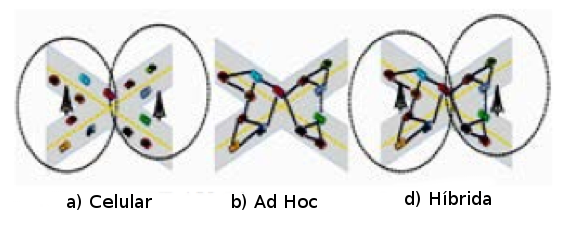
\includegraphics[scale=0.4]{referencial/figuras/Figure28.png}
	\caption{Tipos de VANET \cite{Kumar:2011}.}
	\label{fig:fig28}
\end{figure}

De acordo com \cite{Piran:2011}, com a utilização de sensores nos veículos podem ser desenvolvidos aplicações de dois tipos:

\begin{description}
\item[Aplicação para Segurança:] são utilizadas para reduzir os acidentes envolvendo veículos por exemplo monitorar velocidade, notificação de acidente, notificação de perigo na estrada e alerta de colisão.

\item[Aplicação para Segurança:] são utilizados como para o conforto dos condutor do veículos  por exemplo para notificações de roubo, de congestionamento, de multas de trânsito e informações sobre o tráfico de veículos em um determinado trajeto.
\end{description}

O desempenho de uma VANET pode ser afetado pela topologia da rede que é alterada frequentemente \cite{Lidstrom:2010}, prejudicando o desenvolvimento de aplicações em tempo real por possuir baixo nível de confiança.

\subsection{Sistemas Multi-Agentes}

Segundo \cite{Woolridge:2001}, sistemas multi-agente são sistemas compostos por agentes inteligentes com capacidade de controlar o próprio comportamento e interagir com o ambiente. O autor \cite{Woolridge:2001} sugere que os agentes podem ser agente de software, robôs ou qualquer outro tipo de recurso que realize tarefas.

De acordo com \cite{Woolridge:2001}, os agentes em um sistema multi-agente tem algumas características importantes: 

\begin{description}
\item[Autonomia:] os agentes são pelo menos parcialmente autônomos.

\item[Visão locais:] nenhum agente tem uma visão completa do sistema.

\item[Descentralização:] não há nenhum agente designado para controlar.

\end{description}

O agente possui um conjunto de tarefas para serem executadas nos nós de uma rede. Os nós possuem uma certa capacidade para realizar essas tarefas e também possuem uma quantidade limitada de recursos que podem ser utilizados pelos agentes. Para executar essas tarefas os agentes precisam percorrer a rede para poder acessar os recursos dos nós \cite{Shehory:1998}.

Para \cite{Freitas:2011}, existem duas estratégias para que o agente se locomova sobre a rede. A primeira é através da clonagem dos agentes, enquanto o segundo é chamado de migração dos agentes. Ambos os mecanismos utilizam o mesmo agente que se deslocam pelos nós em uma rede. No entanto, eles se distinguem pelo fato de o agente do primeiro cria uma cópia de si mesmo e este clone é enviado para outro nó, enquanto no segundo, o próprio agente é transmitido para outro nó.


A utilização de um sistema multi-agente sobre VANETs é interessante por que a topologia da rede está em constante mudança, sendo assim é necessário que as escolhas sejam realizadas de acordo com a organização da rede \cite{Freitas:2011}. 

Essas características de sistemas multi-agentes citadas anteriormente tornam a utilização das VANETs mais flexível.  

\subsection{Roteamento geográfico}

Roteamento Geográfico é um conceito de roteamento que se baseia em informações de posição geográfica. Essa organização é propostas para redes sem fio e com base no principio de que a fonte envia uma mensagem para a posição geográfica do destino em vez de usar o endereço de rede \cite{Shu:2010}. 

A utilização de roteamento geográfico em um VANET é sugerida em \cite{Freitas:2011} partindo do principio que o veiculo é maior e possui mais energia facilitando o transporte de um GPS.


Uma importante exigência para a implementação do roteamento geográfico é que cada nó possa determinar sua própria localização e que o emissor esteja ciente da localização do destino. Essas informações são importantes para que os dados transmitidos possam chegar ao destino \cite{Guise:2011}.

Segundo \cite{Taylor:2006}, existem duas técnicas para realizar um roteamento geográfico: 

\begin{itemize}
\item \textbf{Encaminhamento Geográfico}: é um método de roteamento que utiliza a distância geográfica entre dois nós. Os nós simplesmente transmitem pacotes de dados para o seu vizinho mais próximo até o local de destino especificado no pacote. No entanto, este esquema simples pode levar a zonas onde o nó não tem conectividade para região do alvo. 

\item \textbf{Roteamento por Perímetro}: é usado para rotear pacotes em torno das janelas encontrados na rede, assim utilizando alguns algoritmos de grafos para poder contornar essas janelas e atingir os nós que estão no destino.

\end{itemize}

\subsection{Modelo de Movimentos}

Para realizar as simulações nesse trabalho foram utilizados modelos de movimentos, que simulam o comportamento dos nós.

Os modelos de movimentos representam o movimento de componentes móveis, a mudança de sua localização, velocidade e aceleração ao longo do tempo. Tais modelos são frequentemente utilizados para fins de simulação, quando novas técnicas de navegação ou de comunicação são investigados \cite{Nichols:2007}. 

A utilização de modelos de movimentos para realizar simulações em VANET servem para simular os padrões de comportamento dos componentes da rede, por que utilizar componentes reais é inviável \cite{Freitas:2011}.

O autor \cite{Sun:2002} sugere duas abordagens para construir um modelo de movimento:

\begin{itemize}
\item \textbf{Analítico}: esse modelo de movimento é construído por uma fórmula matemática que define os padrões de comportamento dos elementos representados no modelo. 

\item \textbf{Simulado}: é construído através da observação do comportamento dos nós no ambiente que se deseja criar a simulação.

\end{itemize}

\subsection{Simulador GRUBiX}

Para realização das simulações deste trabalho foi utilizado o simulador GRUBiX, que é um simulador open source desenvolvimento na Universidade Federal de Lavras. Ele pode ser encontrado no endereço \url{http://sourceforge.net/projects/grubix/}. Este simulador é uma variação do projeto SHOX \cite{Lessmann:2008}. Assim como o SHOX, o simulador GRUBiX caracteriza-se como um ambiente de simulação orientado a eventos. De forma simplificada, em um ambiente de simulação orientado a eventos, a linha do tempo de uma simulação é representada por uma lista de eventos, em que cada novo evento é inserido nesta lista. A posição em que cada evento é inserido nesta lista varia de acordo com o momento em que cada evento deve ocorrer.

Adicionalmente, estes simuladores oferece um conjunto de ferramentas para que se possa desenvolver toda a pilha de protocolos presente em um equipamento com rede sem fios. Essa disponibilidade permite que cada camada da pilha de protocolos seja personalizada de acordo com as necessidades de cada aplicação.

Assim como o SHOX, o simulador GRUBiX utiliza a linguagem de programação Java. O uso de uma linguagem orientada a objetos, nesse caso Java, indica que as camadas da pilha de protocolos sejam modeladas como objetos. O uso da orientação a objetos permite que cada camada seja personalizada através de mecanismos de herança. Portanto, basta que a nova camada personalizada herde as funcionalidade de uma camada base para que se tenha a possibilidade de alterar o seu comportamento padrão.

\subsection{Padrão ZigBee}

O ZigBee é um padrão de radio frequência que tem como objetivo a padronização e a interoperabilidade de produtos. Ele foi criado e é mantido por um grupo de empresas denominado ZigBee Alliance \cite{ZigBeeAlliance:2015}. O nome ZigBee é uma analogia da forma que as abelhas transitam entre as flores \cite{Safaric:2006}.
A especificação é a IEEE 802.15.4 na camada física e na \emph{Medium Access Control} (MAC) e para camada de rede e aplicação utiliza o ZigBee. Essa pilha pode ser observada na Figura \ref{fig:pilhaZigbee}.

\begin{figure}[htbp]
	\centering
		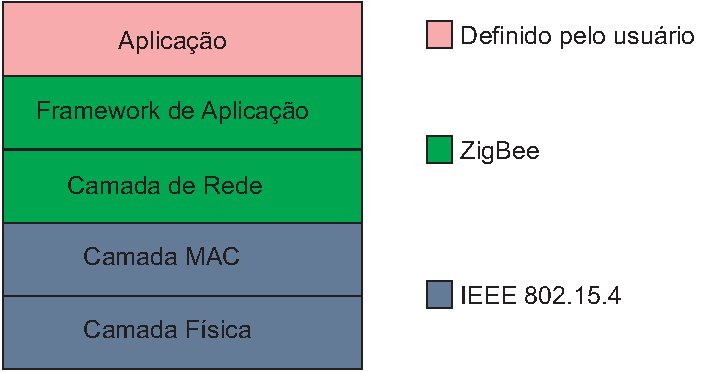
\includegraphics[scale=0.6]{referencial/figuras/pilhaZigbee.pdf}
	\caption{Pilha de protocolo ZigBee.}
	\label{fig:pilhaZigbee}
\end{figure}

Segundo \cite{Ramya:2011}, as principais características do padrão ZigBee são:


\begin{itemize}
  \item Auto reparação.
  \item Suporte a muitos nós.
  \item Facilidade de implementação.
  \item Baixo consumo de energia.
  \item Padrão aberto.
\end{itemize}

\subsection{Arduíno}

O Arduíno é uma plataforma aberta composta por hardware e software. Geralmente são construídos com controladores Atmel AVR de 8 bits. O Arduino pode ser interligados a outros módulos através de hardwares denominados \emph{shields} \cite{Arduino:2015}.

Nesse trabalho é utilizado o modelo Uno \ref{fig:arduinoUno}, que possui um microcontrolador Atmel ATmega 328p com CPU operando a 16MHz. Oferece quatorze portas de entrada e saída, 32kb de memória de programa, 2Kb de SRAM e duas interrupções externas que são mapeadas pelos pinos 2 e 3 da placa. A comunicação com periféricos externos é realizada de forma serial através de uma porta USB \cite{Arduino:2015}.

\begin{figure}[htbp]
	\centering
		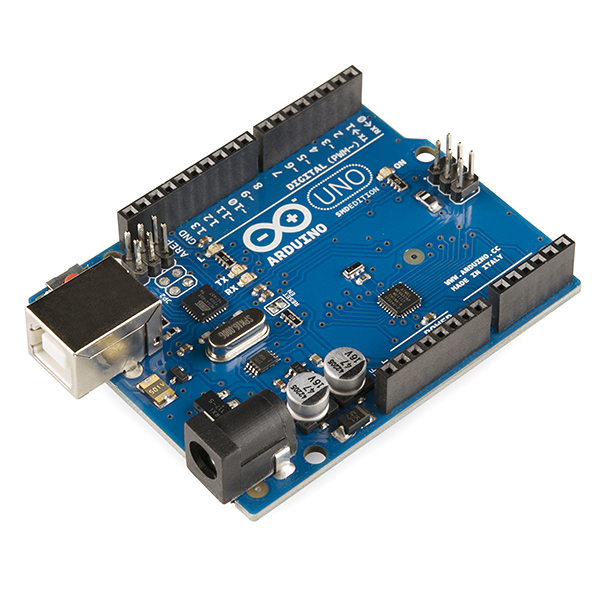
\includegraphics[scale=0.2]{referencial/figuras/arduinoUno.jpg}
	\caption{Arduino UNO.}
	\label{fig:arduinoUno}
\end{figure}

Para programar o Arduino utiliza-se C ou C++. Ele também possui uma IDE demonstrado na Figura \ref{fig:arduinoIde}, com editor de texto e também responsável por carregar o programa na placa do Arduino.

\begin{figure}[htbp]
	\centering
		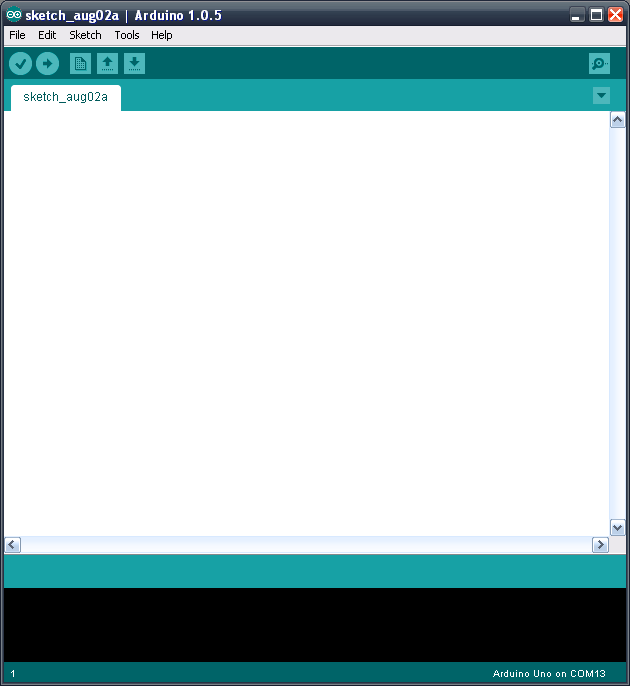
\includegraphics[scale=0.2]{referencial/figuras/arduinoIde.png}
	\caption{Arduino IDE.}
	\label{fig:arduinoIde}
\end{figure}

Para realizar a comunicação esse trabalho utiliza um \emph{shield} para integrar com o módulo Xbee denominado \emph{Xbee shield}.  

\subsection{Trabalhos relacionados}

No trabalho \cite{santanaMestrado:2014}, utiliza-se o protocolo ZigBee para desenvolver uma mecanismo para evitar colisão. O Zigbee é utilizado para enviar aos vizinhos a posição geográfica do veículo obtida através de um dispositivo android. Quando o dispositivo identifica uma possível colisão ele emite um alerta. Para identificar a colisão o disposivo utiliza a longitude e latitude do veículo, a precisão e velocidade. Essas informações são transmitidas pelos vizinhos utilizando o ZigBee.

Os testes realizados por \cite{santanaMestrado:2014} obtiveram uma latência máximo de 65 ms. Com esse resultado mostra que o padrão ZigBee atende aos requisitos de latência para rede veiculares.



O trabalho de \cite{Freitas:2011} analisa a utilização de agentes sensitivos a posição geográficas com diferentes niveis de inteligência. Nele são simulados três níveis de inteligência dos agentes. Os resultados das simulações fornecem informações sobre a importância do uso do contexto para que os agentes possam cumprir a sua missão. 



\label{sec:metodologiaSimulacao}

Após examinar diversos artigos e trabalhos científicos que abordaram redes veiculares, não foi identificado um padrão metodológico para a avaliação dessas redes. Normalmente, cada autor realiza a metodologia de acordo com as variáveis que se deseja avaliar. 

O uso de simulação justificou-se pela complexidade em se aplicar as técnicas propostas em uma grande quantidade de veículos, questões financeiras e relacionadas ao tempo para se testar o algoritmo em uma grande variedade de cenários também foram avaliadas.

\subsection{Simulação}
\label{subsec:simulacao}

O desenvolvimento da simulação foi dividido em três etapas. A primeira etapa é a construção do cenário com o modelo de movimento, veículos e infraestrutura. A segunda etapa é o desenvolvimento dos agentes de software, e por último a fase de simulação. 

A simulação foi desenvolvida utilizando o simulador GRUBiX e executada em um notebook com configuração detalhada na tabela \ref{tab:configuracaoNotebook}.

\begin{table}[ht]
	\caption{Configuração do notebook utilizado nas simulações}
	\centering
	\begin{tabular}{|l|l|}
		\hline
		Sistema Operacional & Ubuntu Linux 10.10 \\ \hline
		Processador & Intel Core i7-2630QM 2.00GHz (6M Cache) \\ \hline
		Memória RAM & 8GB SSD \\ \hline
		Disco Rígido & 120 GB SSD \\ \hline 
	\end{tabular}

	\label{tab:configuracaoNotebook}
\end{table}

\subsubsection{Cenário}

O cenário é uma cidade dividida em quadras seguindo o modelo de movimento \emph{Manhattan}. Nessa cidade possuem veículos que percorrem as quadras. Alguns cruzamentos possuem uma infraestrutura e elas estão conectadas através de cabos. 

A figura \ref{fig:modeloMovimentoManhattan} apresenta um esboço do cenário onde pode-se observar as ruas, os veículos e a infraestrutura. Esse cenário é utilizado em todas simulações, entretanto a infraestrutura é desativada quando não é utilizada.

\begin{figure}[htbp]
	\centering
	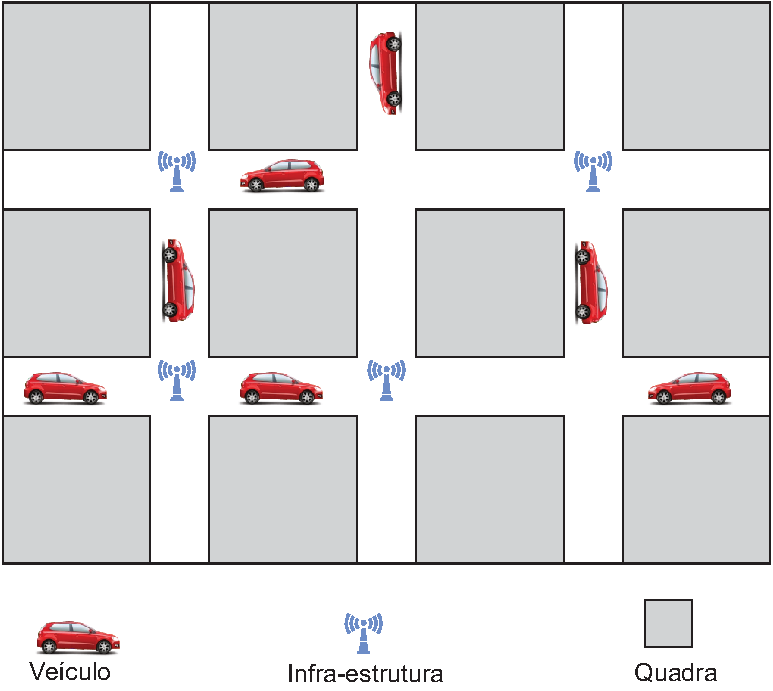
\includegraphics[scale=0.7]{metodologia/figuras/modeloMovimentoManhattan.pdf}
	\caption{Modelo de cidade utilizado.}
	\label{fig:modeloMovimentoManhattan}
\end{figure}

O comprimento e a largura da região de simulação são levados em consideração na construção do cenário. As linhas horizontais e verticais são as ruas e o cruzamento delas são as quadras. Para obter a quantidade de ruas horizontais e verticais são utilizadas as Equações \ref{eq:equacaoQuantidadeRuasHorizontal} e \ref{eq:equacaoQuantidadeRuasVertical}.

\begin{equation}
	\label{eq:equacaoQuantidadeRuasHorizontal}
	Q_{rh} = {A_{at} \over A_{aq}}
\end{equation} 

\begin{tabular}{ l c r} 
	Onde:\\
	Q\tiny rh \normalsize= quantidade de ruas na horizontal \\
	A\tiny at \normalsize= altura total do cenário \\
	A\tiny aq \normalsize= altura das quadras\\
\end{tabular}

\begin{equation} 
	\label{eq:equacaoQuantidadeRuasVertical}
	Q_{rv} = {L_{lt} \over L_{lq}} 
\end{equation}

\begin{tabular}{ l c r}
	Onde:\\ 
	Q\tiny rh \normalsize= quantidade de ruas na vertical \\
	L\tiny lt \normalsize= largura total do cenário \\
	L\tiny lq \normalsize= largura das quadras\\
\end{tabular}

\paragraph{Veículos e infraestrutura}

O agente necessita que os nós (veículos e a infraestrutura) tenham dois recursos fundamentais para o seu funcionamento: a capacidade de comunicação; e o agente deve conseguir executar suas instruções. Na simulação todos os nós possuem essa competência.

Quando um agente chega em um nó, ele logo executa a suas instruções. No simulador o nó executa um evento para verificar se existe algum agente hospedado nele. Se existir o evento retorna um objeto que deve implementar a interface agente que se encontra no Anexo \ref{app:agente}. Com o objeto o nó executa o método \texttt{execute()}. As classes do programa em Java  que simulam o comportamento do nó se encontra no Anexo \ref{app:comportamentoNo}. O Anexo \ref{app:movimento} descreve a classe java que implementa o modelo de movimento.

Todos os veículos e infraestruturas possuem o mesmo comportamento em relação ao agente. Por outro lado, eles possuem comportamentos diferentes em relação ao ambiente. Primeiramente os veículos possuem a capacidade de locomoção. Embora a infraestrutura não possua essa capacidade, todas elas estão conectadas. Em outras palavras, quando um agente está em uma infraestrutura ele não consegue se locomover porém consegue se comunicar com todas as outras infraestruturas espalhadas pelo cenário. 

Ao iniciar a simulação os veículos e as infraestruturas são distribuídos entre os cruzamentos de maneira aleatória. 

O Algoritmo \ref{lst:algoritmoComportamentoNos} de locomoção leva em consideração a equação da reta que representa a rua. Isto significa que quando o veículo está em uma rua do tipo horizontal ele se movimenta em \emph{X} e quando estiver em uma rua do tipo vertical o veículo se movimenta em \emph{Y}. Para simular a velocidade quando um veículo entra em uma rua, o tipo dela é verificado e então soma ou subtrai um valor da posição atual dele.

\begin{algorithm}
	\scriptsize
	\Inicio{
		$nos \gets pegarListaNos()$\;
		$i \gets 0$\;
		\Repita{i == nos.length}{
			\uIf{nos[i].eVeiculo()}{
				pontoProximoCruzamento = nos[i].pegarCruzamentoMaisProximo()\;
				distancia = pontoProximoCruzamento.calcularDistancia(nos[i].posicao)\;
				\uIf{distancia < nos[i].velocidade}{
					nos[i].velocidade = distancia\;
				}
				\Else{
					\uIf{distancia == 0}{
						nos[i].mudarDirecao()\;
					}
					\Else{
						nos[i].andar()\; 
					}
				}
			}
			\uIf{nos[i].possuiAgente()}{
				nos[i].pegarAgente().execute()\;
			}
			i++\;
		} 
	}
	\caption{Algoritmo movimento dos nós.}
	\label{lst:algoritmoComportamentoNos}
\end{algorithm} 

Quando a velocidade do veículo é maior que a distância entre a posição atual dele e de um cruzamento, a sua velocidade diminui até chegar em zero. Isto significa que o veículo chegou em um cruzamento, então o veículo deve decidir entre continuar, virar para esquerda, virar para direita ou voltar. Cada direção possui uma probabilidade como demonstra a Tabela \ref{tab:probabilidadeEscolhaDirecao}.

No caso da infraestrutura a velocidade é sempre zero. Assim elas utilizam o mesmo algoritmo dos veículos porém não mudam de posição.

\begin{table}[ht]
	\caption{Probabilidade do veículo escolher uma direção}
	\centering
	\begin{tabular}{ | l | c | r}
		\hline
		Frente & 50\% \\ \hline
		Direita & 20\% \\ \hline
		Esquerda & 20\% \\ \hline
		Voltar & 10\% \\ \hline 
	\end{tabular}
	\label{tab:probabilidadeEscolhaDirecao}
\end{table}

O Algoritmo \ref{lst:algoritmoAproximacaoRuas} demonstra que em cada movimento do veículo são calculadas as distâncias entre a sua posição atual e de todos os cruzamentos contrários ao tipo de rua que o veículo está locomovendo.
Por exemplo, quando um veículo se locomove em uma rua horizontal, a cada movimento o algoritmo calcula as distâncias entre a posição do veículo e as ruas verticais.

\begin{algorithm}
	\scriptsize
	\Inicio{
		\Entrada{O nó a ser testado}
		$i \gets 0$\;
		\uIf{no.tipoRua == horizontal}{
			$y \gets no.posicao.getY()$\;
			\Repita{$i < Q_{rh}$}{
				$y_{rua} \gets A_{aq}(1 + i)$ \;
				\uIf{$y_{rua} - y < no.velocidade$}{
					retorna $y_{rua} - y$ \;
				}
				i++\;
			}
		}
		\Else{
			\uIf{no.tipoRua == vertical}{
				$x \gets no.posicao.getX()$\;
				\Repita{$i < Q_{rv}$}{
					$x_{rua} \gets L_{lq}(1 + i)$ \;
					\uIf{$x_{rua} - x < no.velocidade$}{
						retorna $x_{ruax} - x$ \;
					}
					i++\;
				}
			}
		} 
	}
	\caption{Algoritmo que identifica a aproximação com um cruzamento.}
	\label{lst:algoritmoAproximacaoRuas}
\end{algorithm}

Para definir as ruas horizontais é utilizado a Equação \ref{eq:equacaoParaEncontraRuasHorizontais} que é a equação da reta quando a reta cruza o eixo \emph{Y}.

A Equação \ref{eq:equacaoParaEncontraRuasVerticais} é utilizada para definir as ruas verticais. Todas as ruas horizontais se cruzam com as ruas verticais, então para descobrir um cruzamento é necessário indicar o número da rua nas Equações \ref{eq:equacaoParaEncontraRuasHorizontais} e \ref{eq:equacaoParaEncontraRuasVerticais} respectivamente. Com isso é optido um ponto que corresponde ao cruzamento.

\begin{equation} 
	\label{eq:equacaoParaEncontraRuasHorizontais}
	Y = A_{aq}(1+N_{horizontral}) 
\end{equation}

\begin{tabular}{ l c r}
	Onde:\\ 
	Y = posição da rua \\
	A\tiny aq \normalsize= altura das quadras\\
	N\tiny horizontal \normalsize=número de quadras onde $N_{horizontal} \in I, 0 \leq N_{horizontal} < Q_{rv}$\\
\end{tabular}

\begin{equation} 
	\label{eq:equacaoParaEncontraRuasVerticais}
	X = L_{lq}(1+N_{vertical}) 
\end{equation}

\begin{tabular}{ l l}
	Onde:\\ 
	X = posição da rua \\
	L\tiny lq \normalsize= largura das quadras\\
	N\tiny vertical \normalsize=número de quadras onde $N_{vertical} \in I, 0 \leq N_{vertical} < Q_{rv}$\\
\end{tabular}

\subsubsection{Agente de Software}

Foi utilizado \cite{Freitas:2011} como referência para a construção do agente de software. A missão do agente é permanecer dentro de uma região (região alvo) no cenário. A região é definida por dois pontos, sendo um limite superior e outro o limite inferior, como demonstra a Figura \ref{fig:regiaoAlvo}. 

\begin{figure}[htbp]
	\centering
	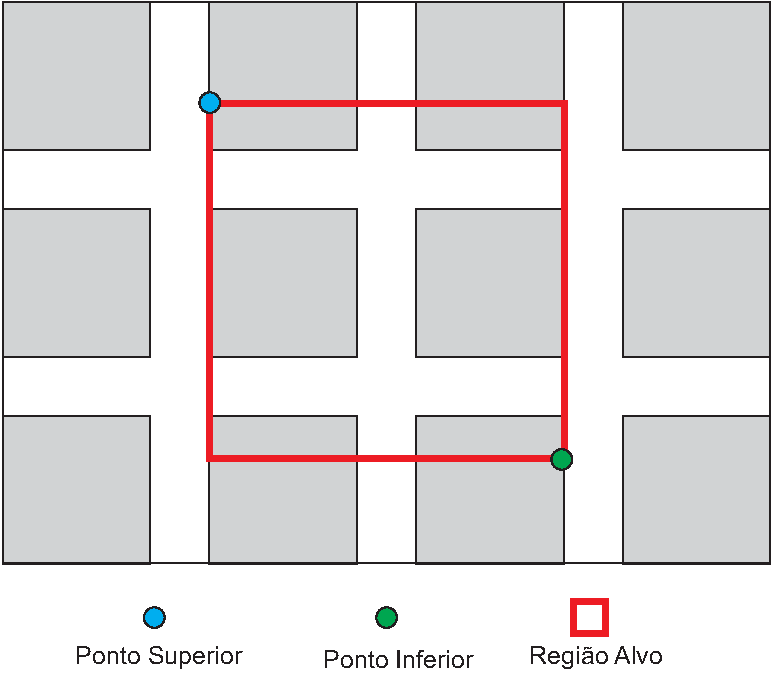
\includegraphics[scale=0.7]{metodologia/figuras/regiaoAlvo.pdf}
	\caption{Região Alvo.}
	\label{fig:regiaoAlvo}
\end{figure}

Para a simulação foram criados dois tipos de agentes. O agente que deve se manter dentro da região alvo é o agente principal. O agente principal pode criar um tipo de agente mais simples, o \emph{mini-agente}, que é responsável por buscar nós que possam propiciar ao agente principal maior possibilidade de finalizar a sua missão.

Quando a simulação inicia é escolhido um nó aleatoriamente para receber um agente principal. Então o nó executa as instruções do agente. Para o funcionamento dessa arquitetura o agente precisa possuir uma interface onde o veículo consiga acessar as instruções do agente. Os nós também devem ter uma interface onde o agente consiga acessar recursos necessários para o seu funcionamento. Nesse trabalho, os nós possuem três recursos disponíveis:

\begin{itemize}
	\item Posição atual
	\item Posição com o destino do nó
	\item Comunicação com os nós vizinhos
\end{itemize} 

Na Figura \ref{fig:umlAtores} pode-se visualizar a arquitetura das simulações. Essa arquitetura permite adicionar mais atores na simulação, por exemplo, agentes como missões diferentes ou até mesmo uma pessoa com algum equipamento que permita o transporte dos agentes. Assim, possibilita-se ao agente acessar regiões antes impossíveis para acesso de veículos. 

\begin{figure}[htbp]
	\centering
	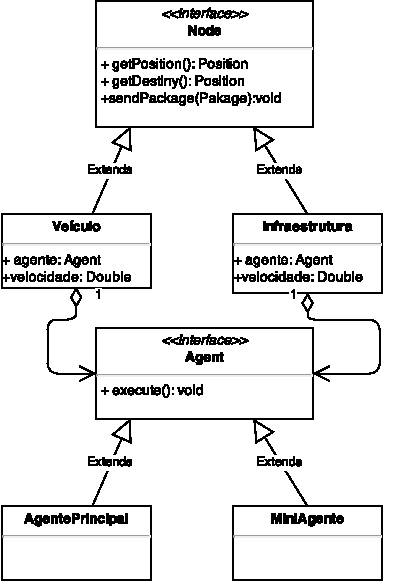
\includegraphics[scale=0.8]{metodologia/figuras/umlAtores.pdf}
	\caption{Diagrama UML com a relação entre as entidades.}
	\label{fig:umlAtores}
\end{figure}

A missão do agente é alcançar a região alvo e permanecer nela. Para isto, o agente deve conhecê-la. Então a primeira ação do agente é solicitar ao nó onde ele está hospedado a sua posição. Se o veículo estiver na região alvo o algoritmo termina a sua execução, e nesse momento poderia realizar outras atividades como recolher dados ou disseminar propaganda.

Caso a posição do nó não está no interior da região alvo, o agente precisa procurar um hóspede mais apropriado. Para isso é criado um segundo agente, mais simples que o primeiro, com a missão de procurar entre os nós vizinhos um mais apropriado. O Algoritmo \ref{lst:algoritmoAgentePrincipal} descreve o funcionamento do agente principal.

\begin{algorithm}
	\scriptsize
	\Inicio{
		\Repita{$no.agentePrincipal \neq vazio$}{
			$regiaoAlvo \gets pegarRegiaoAlvo()$\;
			$posicaoNo \gets no.pegarPosicao()$\;
			$destinoNo \gets no.pegarDestino()$\;
			\uIf{$posicaoNo \in regiaoAlvo$}{
				executarTarefasDaRegiaoAlvo()\;
			}
			\Else{
				$miniAgente \gets criarMiniAgente(posicaoNo, destinoNo, regiaoAlvo)$\;
				$mensagem \gets no.enviarMensagem()$\;
				$reposta = escutarReposta(mensagem)$\;

				\uIf{reposta = vazio}{
					executarTarefasForaRegiaoAlvo()\;
				}
				\Else{
					no.enviarMensagem(agentePrincipal, reposta.idImovelSelecionado())\;
				}
			}
			hibernarPeriodo()\; 
		} 
	}
	\caption{Algoritmo do Agente Principal.}
	\label{lst:algoritmoAgentePrincipal}
	\end{algorithm}

Cada nó vizinho recebe uma cópia do \emph{mini-agente} e o executa. Na estrutura do \emph{mini-agente} contém a região alvo e a distância do destino com a região alvo. Esses dados são comparados pelo \emph{mini-agente} com os dados dos nós que o receberam. Caso algum nó tenha uma condição melhor que o nó onde o agente principal está hospedado o \emph{mini-agente} envia um sinal avisando o agente principal para ele migrar. Após finalizar a missão o \emph{mini-agente} é descartado. O funcionamento do \emph{mini-agente} é reproduzido pelo algoritmo \ref{lst:algoritmoMiniAgente}.

\begin{algorithm}
	\scriptsize
	\Inicio{
		\Entrada{posicaoNoHospedeiro, destinoNoHospedeiro, regiaoAlvo}
		$distanciaRegiaoAlvoDestinoNoHospedeiro \gets regiaoAlvo.calcularDistancia(destinoHospedeiro)$\;
		$distanciaRegiaoAlvoDestinoNo \gets regiaoAlvo.calcularDistancia(no.destino)$\;
		\uIf{$no.posicao \in regiaoAlvo$}{
			no.enviarSinal(no.id)\;
		}
		\Else{

			\uIf{$no.destino \in regiaoAlvo$}{
				no.enviarSinal(no.id)\;
			}
			\Else{
				\uIf{$distanciaRegiaoAlvoDestinoNoHospedeiro < distanciaRegiaoAlvoDestinoNo$}{
					no.enviarSinal(no.id)\;
				}
			}
		}
		no.removerMiniAgente()\;s
	}
	\caption{Algoritmo do Mini-agente.}
	\label{lst:algoritmoMiniAgente}
\end{algorithm}

Durante a seleção três perguntas devem ser respondidas e, se uma das respostas for afirmativa, o \emph{mini-agente} envia o sinal para o agente principal migrar:

\begin{enumerate}
	\item Nó está dentro da região alvo? (Figura \ref{fig:veiculoSelecionadoDentroRA})
	\item Destino do nó é dentro da região alvo? (Figura \ref{fig:destinoVeiculoSelecionadoDentroRA})
	\item Destino do nó é mais próximo da região alvo? (Figura \ref{fig:destinoVeiculoSelecionadoProximoRA})
\end{enumerate}

\begin{figure}[htbp]
	\centering
	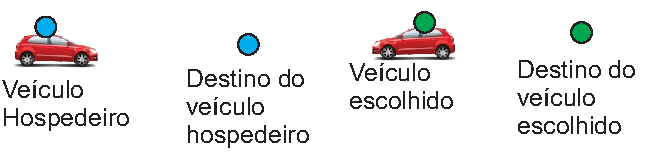
\includegraphics[scale=0.7]{metodologia/figuras/legendaSelecaoMelhorVeiculo.pdf}
\end{figure}

\begin{figure}[htbp]
	\centering
	\begin{minipage}{0.50\textwidth}
		\centering
		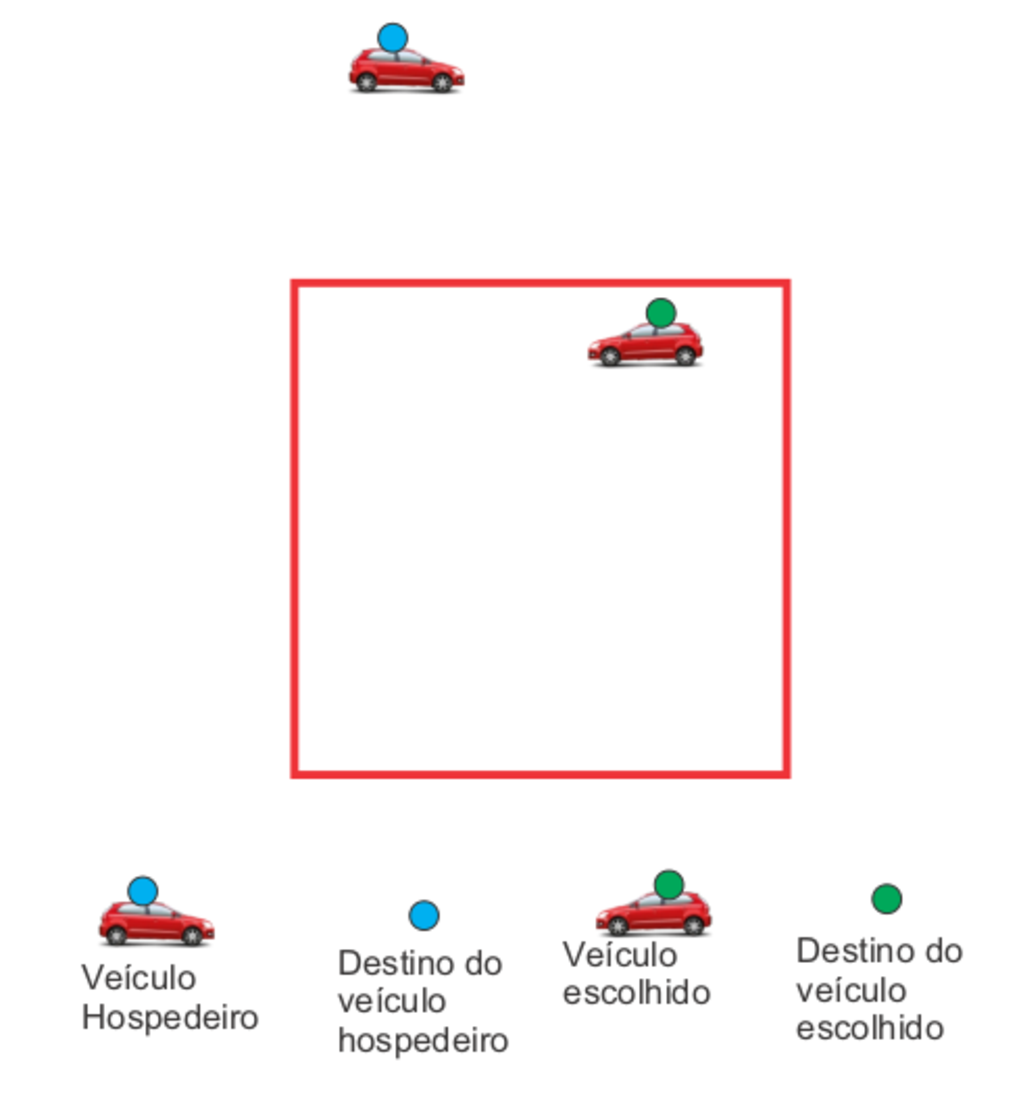
\includegraphics[scale=0.5]{metodologia/figuras/veiculoSelecionadoDentroRA.pdf}
		\captionof{figure}{Veículo dentro da Região Alvo.}
		\label{fig:veiculoSelecionadoDentroRA}
	\end{minipage}%
	\begin{minipage}{0.50\textwidth}
		\centering
		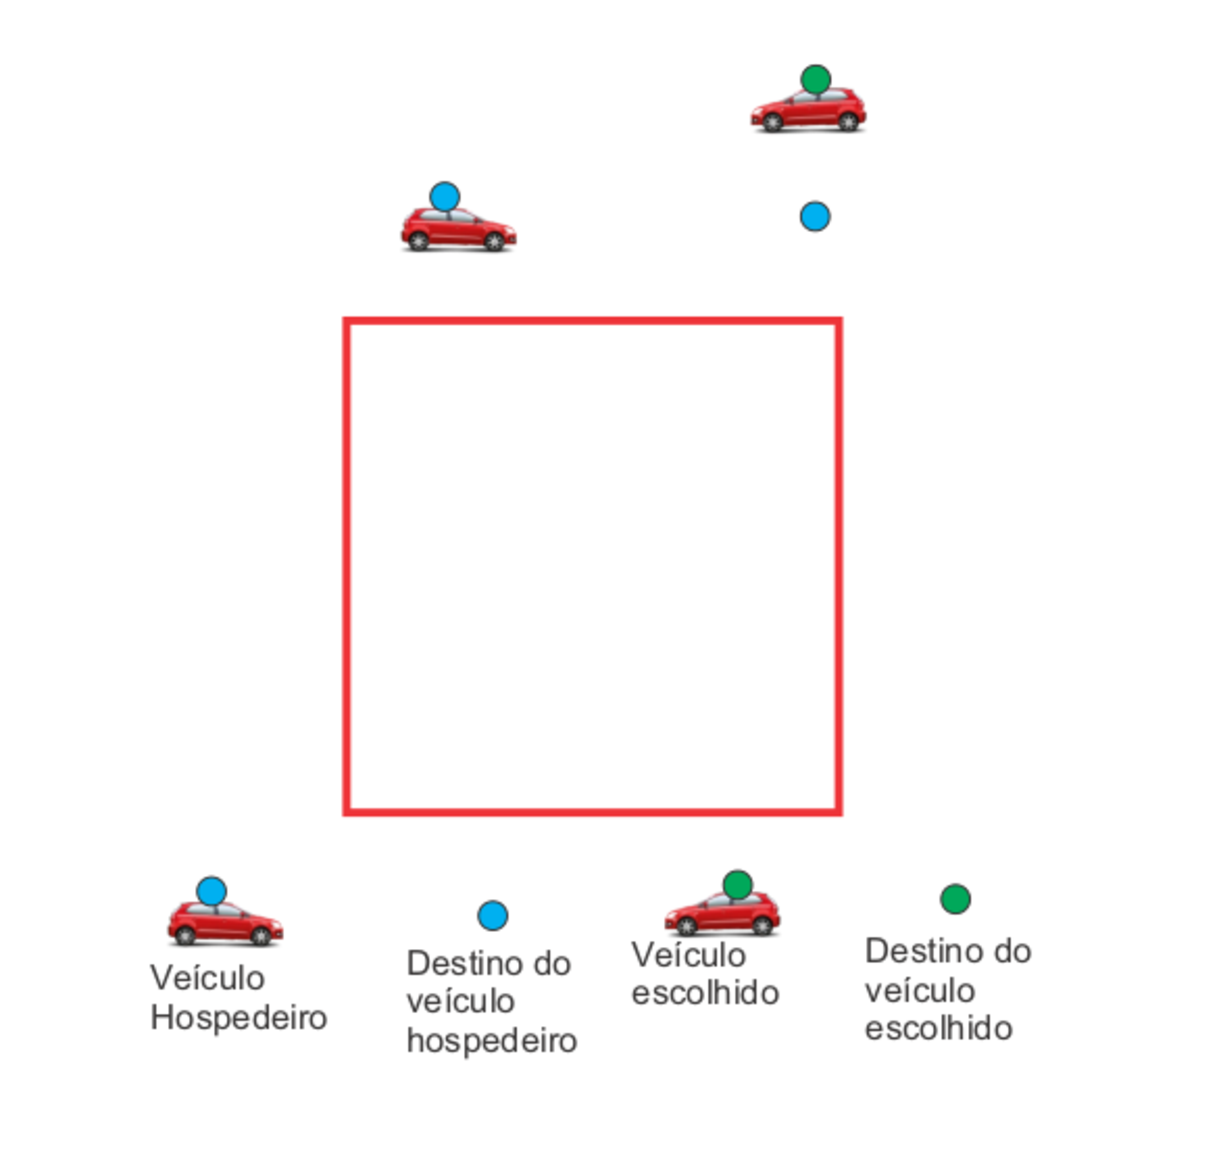
\includegraphics[scale=0.5]{metodologia/figuras/destinoVeiculoSelecionadoDentroRA.pdf}
		\captionof{figure}{Destino veículo dentro da Região Alvo.}
		\label{fig:destinoVeiculoSelecionadoDentroRA}
	\end{minipage}
	\begin{minipage}{0.50\textwidth}
		\centering
		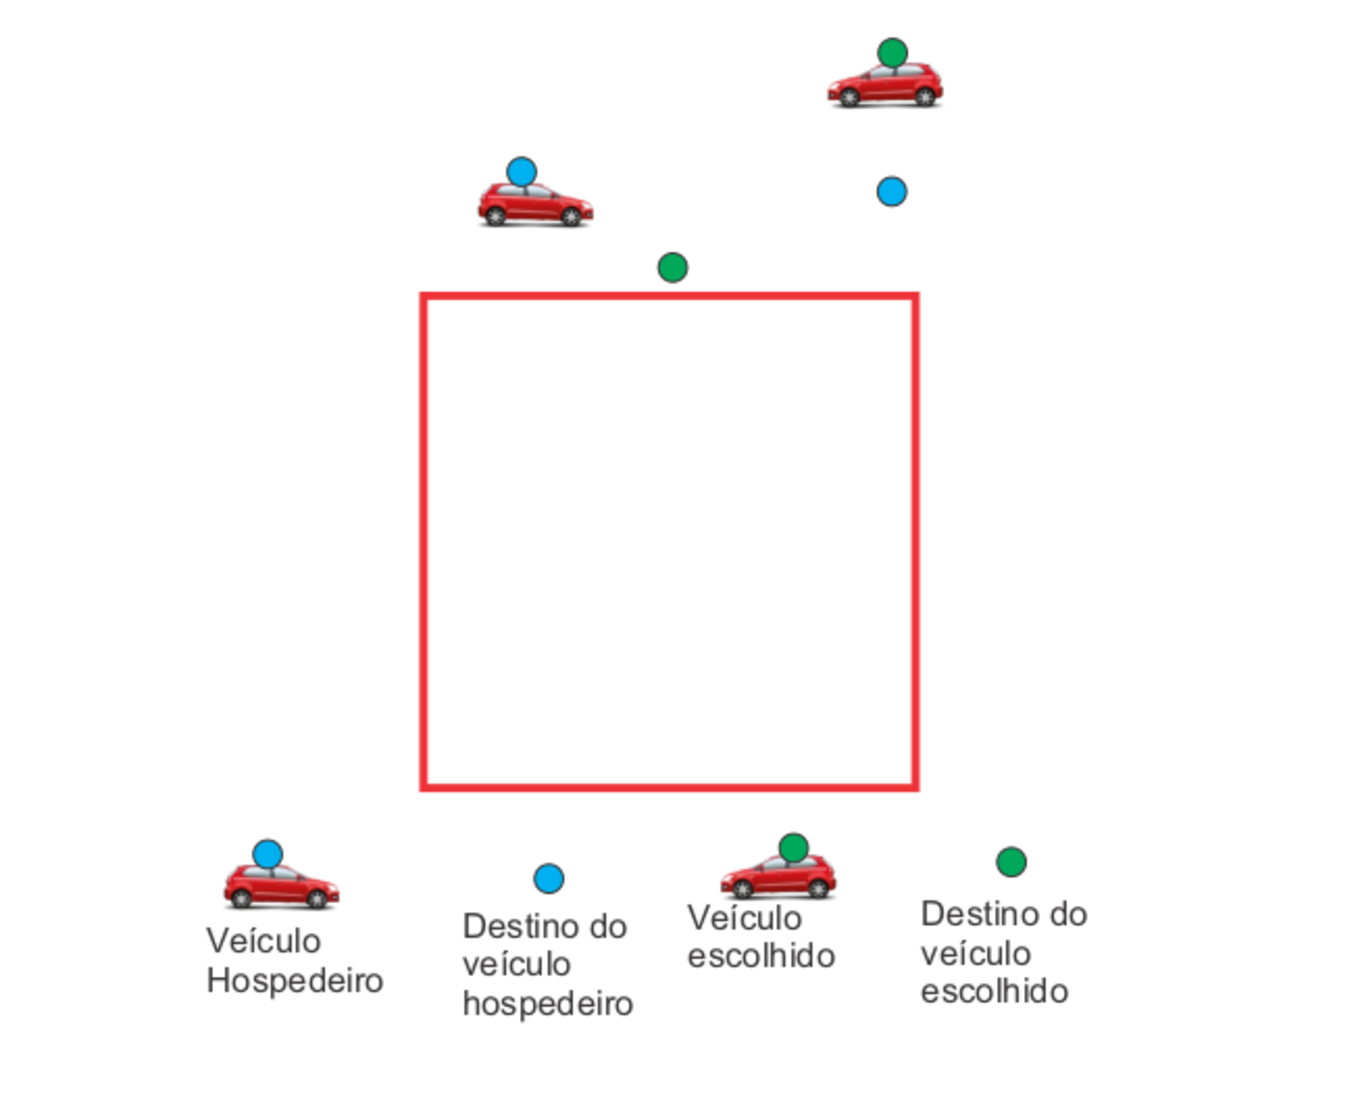
\includegraphics[scale=0.5]{metodologia/figuras/destinoVeiculoSelecionadoProximoRA.pdf}
		\captionof{figure}{Destino do veículo selecionado dentro da Região Alvo.}
		\label{fig:destinoVeiculoSelecionadoProximoRA}
	\end{minipage}
\end{figure}

O primeiro sinal que alcançar o agente principal, ele realiza a migração para o nó que enviou o sinal. Essa abordagem é utilizada por dois motivos:

\begin{description}
	\item[Primeiro:] O sinal contendo somente o identificador do nó possui poucos bytes.
	\item[Segundo:] Elimina a necessidade do desenvolvimento um mecanismo para esperar que todos os \emph{mini-agente} executem a sua missão e só depois tomar a decisão de escolher o melhor nó.
\end{description}

Na simulação que a infraestrutura está ativada, ela pode replicar o \emph{mini-agente} para todos os outros nós próximos 
às infraestruturas espalhadas pelo cenário, aumentando a abrangência da busca. Se um nó distante for escolhido, o agente principal pode utilizar a infraestrutura para alcançá-lo. A Figura \ref{fig:exemploComInfraestrutura} demonstra uma situação onde o \emph{mini-agente} encontra uma infraestrutura.

\begin{figure}[htbp]
	\centering
	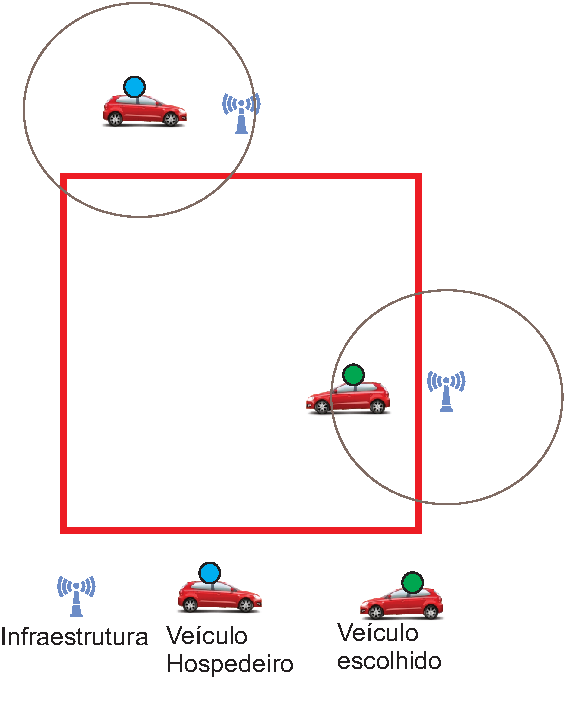
\includegraphics[scale=0.5]{metodologia/figuras/exemploComInfraestrutura.pdf}
	\label{fig:exemploComInfraestrutura}
	\caption{Exemplo com infraestrutura.}
\end{figure}

Para não congestionar a rede, o agente principal deve evitar procurar novos nós por um período de tempo, e durante esse período ele pode executar outras tarefas. Esse comportamento pode ser repetido infinitamente ou o agente pode ter um tempo determinado para executar a sua missão. Ao fim desse tempo, o agente deixa de existir.

\subsubsection{Realizar simulação}

O objetivo da simulação é averiguar se a adição de uma infraestrutura melhora a locomoção dos agentes de software, favorecendo que ele desempenhe a sua missão. Após o desenvolvimento e testes do cenário e de todos os atores da simulação é necessário configurar o simulador. As varáveis que o simulador GRUbiX utiliza são: quantidade dos nós, alcance do sinal, largura e altura do cenário. 

As variáveis largura e altura do cenário são constantes em 120 metros. Por outro lado, a quantidade de nós e alcance de cada nó são variáveis. Essa variação permite simular o comportamento do agente em ambientes com alta e baixa densidade de veículos. Com a altura e largura do cenário é possível obter as quadras. Elas possuem 10 metros de altura e 10 de largura, totalizando 144 quadras.

Após configurar as variáveis de ambiente do GRUBiX é necessário configurar os atores da simulação. Os atores da simulação são: veículos, infraestruturas, agente principal e o agente secundário. As variáveis dos nós que representam os veículos são o alcance e a velocidade. Os nós que representam as infraestruturas possuem o mesmo alcance dos veículos, porém a velocidade é nula e também podem ser ativados e desativados. O agente principal só precisa conhecer a região alvo, onde o ponto superior é S(80,100) e o inferior é I(100,80) sendo a escala em metros.  

Então foram modeladas vinte e quatro situações para serem simuladas. Elas consistem em doze com a infraestrutura ligada e outras doze com a infraestrutura desligada. A Tabela \ref{tab:resumoConfiguracaoSimulacao} apresenta um resumo das configurações simuladas. 

\begin{table}[ht]
	\caption{Resumo das configurações da simulação}
	\centering
	\begin{tabular}{| l | l | l | l | l | l | l | l | l |}
		\hline
		Infraestrutura & \multicolumn{4}{|c|}{Ativada} & \multicolumn{4}{|c|}{Desativada} \\ \hline
		Quantidade de nós & 25 & 50 & 75 & 100 & 25 & 50 & 75 & 100 \\ \hline
		Alcance dos nós (metros) & 5 & 5 & 5 & 5 & 5 & 5 & 5 & 5 \\
		Alcance dos nós (metros)& 10 & 10 & 10 & 10 & 10 & 10 & 10 & 10 \\
		Alcance dos nós (metros)& 15 & 15 & 15 & 15 & 15 & 15 & 15 & 15 \\
		\hline 
	\end{tabular}
	\label{tab:resumoConfiguracaoSimulacao}
\end{table}

O simulador permite uma visualização da simulação como apresenta a Figura \ref{fig:visulizacaoSimulador}. Nela as linhas representam as ruas, os pontos amarelos são os veículos e os vermelhos são a infraestrutura. Nas simulações, quando a infraestrutura está ativada, cinco nós que seriam veículos se tornam infraestrutura e a sua velocidade mantém nula. Quando a infraestrutura está desligada os nós continuam sendo veículos. Exemplificando: com a infraestrutura ligada, quando existir vinte e cinco nós, cinco nós são infraestrutura e o restante veículos. Por outro lado, quando a infraestrutura estiver desligada, todos os nós são veículos.

\begin{figure}[htbp]
	\centering
	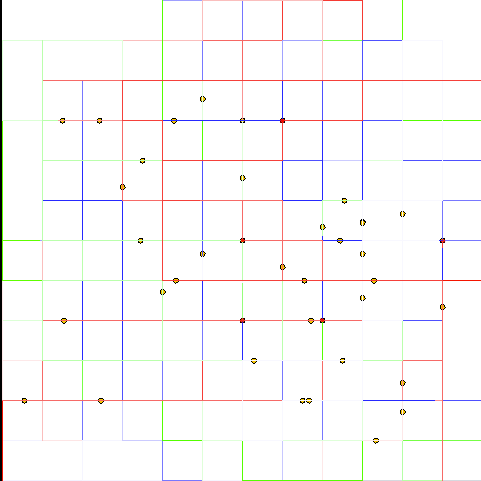
\includegraphics[scale=0.4]{metodologia/figuras/simulacaoGrubix.png}
	\caption{Visualização no simulador.}
	\label{fig:visulizacaoSimulador}
\end{figure}

Foram realizadas mil simulações para cada uma das vinte e quatro situações totalizando vinte e quatro mil simulações. Os dados recolhidos foram o tempo de simulação e o tempo que o agente permaneceu dentro da região alvo.  

Com esses dados é possível obter a porcentagem de tempo que o agente principal permaneceu na região alvo e o impacto que cada variável tem no desempenho do agente em cumprir a missão. Com os resultados finais foram calculados desvio padrão, variância e assim analisados.







%\section{Resultado e Discussão}
\label{sec:resultados}

Os resultados apresentados nesta seção estão divididos em duas partes. A primeira parte abrange as simulações realizadas e os resultados obtidos como é descrito nas Seções \ref{sec:simulacao} e \ref{sec:prototipoExperimento}. A segunda parte abrange o experimento prático realizado na UFLA com estudo da taxa de perda do agente e latência como descrito na Seção \ref{subsec:prototipoExperimento}. 

\subsection{Resultados da Simulação}
\label{subsec:resultadoSimulacao}

	Diversas simulações foram realizadas no simulador GRUBiX, como descrito na Seção \ref{sec:simulacao}. As simulações foram realizadas para avaliar o comportamento do agente em redes com diferentes níveis de densidade de nós e distância de comunicação dos nós. Também foram simuladas redes somente com veículos sem uma infraestrutura de apoio e outra híbrida.

	Após realizar as simulações, os dados foram organizados e analisados em três fases:

	\begin{enumerate}
		\item Resultados obtidos na rede sem infraestrutura.
		\item Resultados obtidos na rede híbrida.
		\item Comparação dos resultados obtidos nas duas situações.
	\end{enumerate} 

	\subsubsection{Rede sem infraestrutura}
	\label{subsubsection:redeSemInfraestruturaResultadoDiscucao}

	Os resultados obtidos da rede sem infraestrutura mostram que o raio de alcance e a quantidade dos nós afetam o desempenho do agente. A Figura \ref{fig:graficosSemTorres} demonstra a evolução do tempo que o agente permaneceu na região alvo (desempenho do agente) com o aumento do raio e a quantidade de nós. 

	\begin{figure}[htbp]
		\centering
		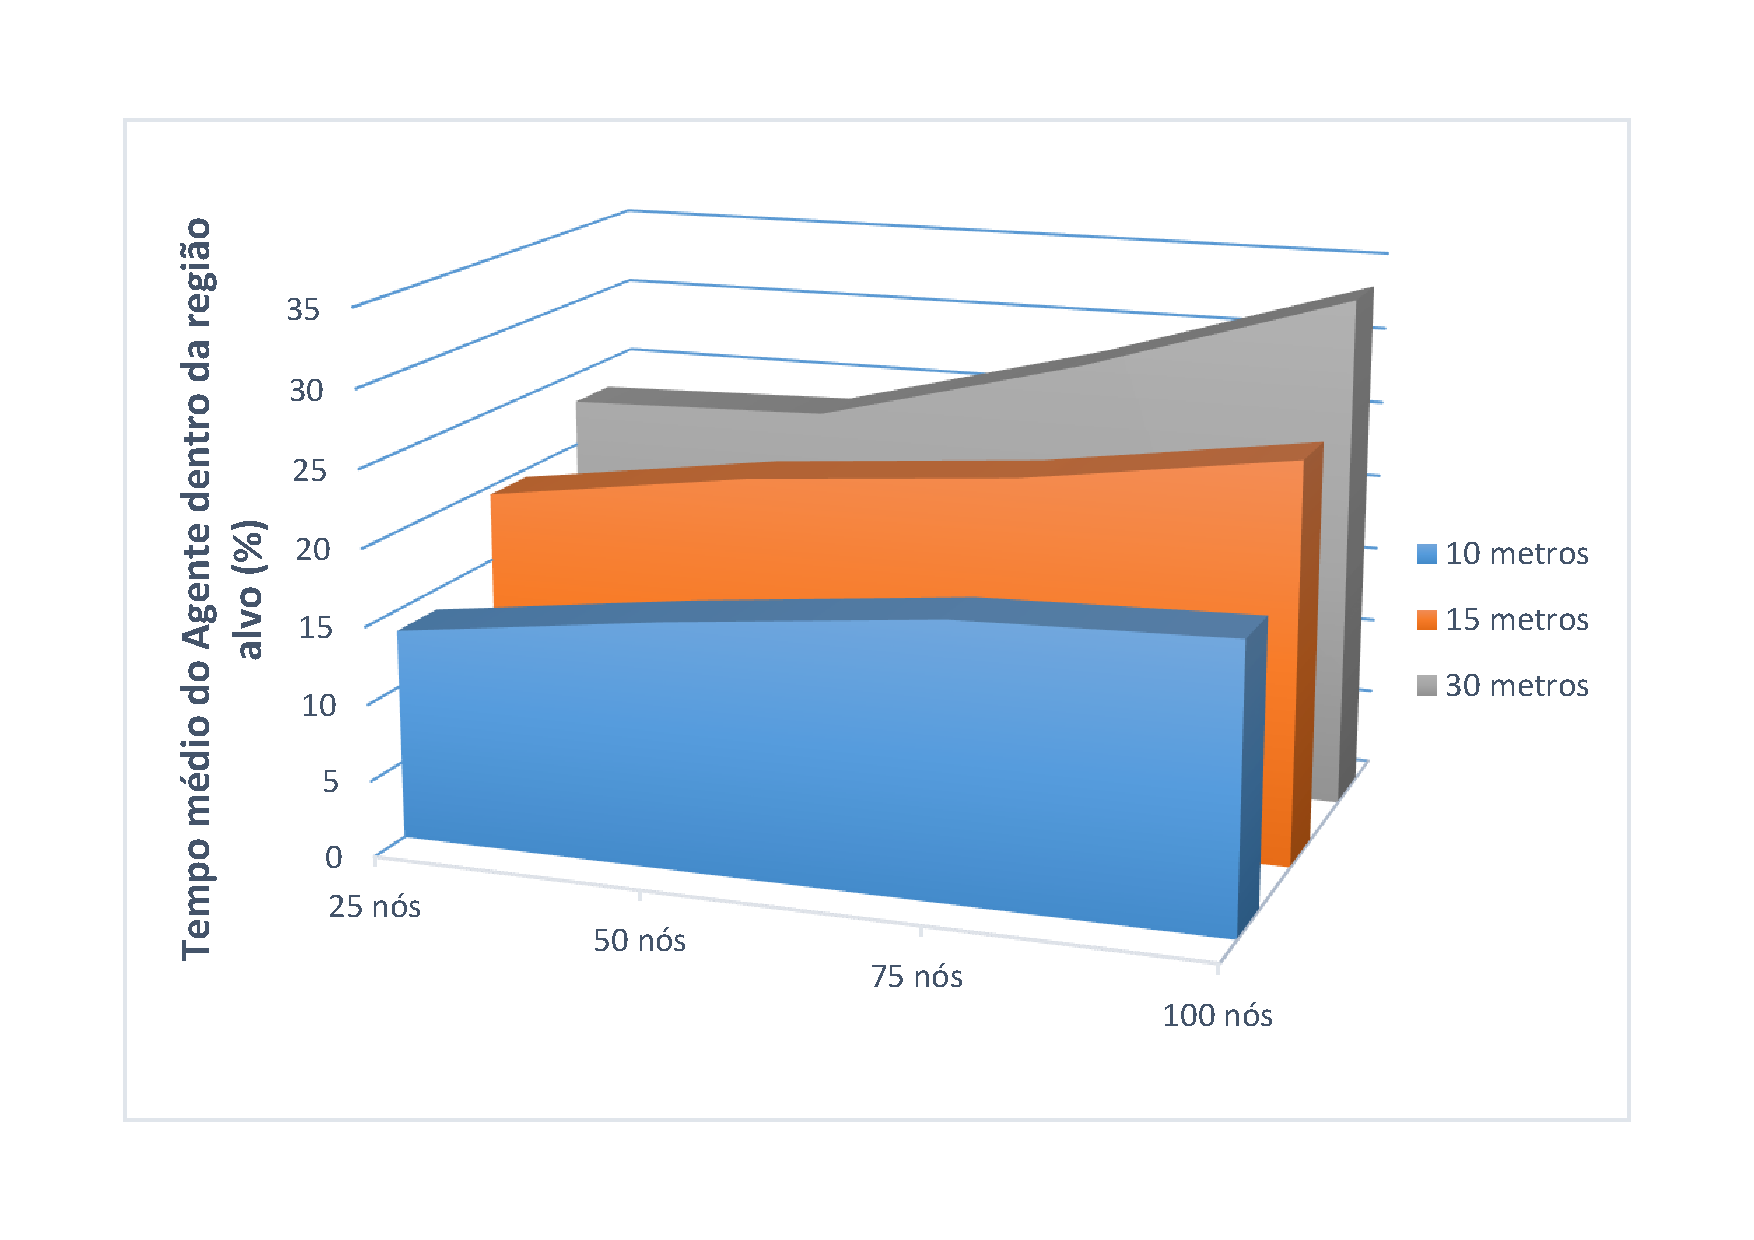
\includegraphics[scale=0.5]{resultados/graficos/graficoSemTorres.pdf}
		\caption{Resultados obtidos nos cenários sem infraestrutura.}
		\label{fig:graficosSemTorres}
	\end{figure}

	Na Tabela \ref{tab:estatiscaResultadosObtidosSemInfraestrutura} é possível visualizar a média aritmética, o desvio padrão e a variância dos resultados obtidos. 

	\begin{table}[!htb]
	    \caption{Estátistica dos resultados obtidos relativos a situação sem infraestrutura.}
	    \label{tab:estatiscaResultadosObtidosSemInfraestrutura}
	    \centering
	    \scriptsize
	    \begin{minipage}{.5\linewidth}
	      
	      \centering
	        \begin{tabular}{|c|c|c|c|}

			\hline
			\multicolumn{3}{|c|}{25 nós} \\ \hline
			Alcance   & média aritmética &	Desvio Padrão  \\ \hline
			10 metros &	13,67 & 2,25  \\ \hline
			15 metros &	19,45 & 1,71   \\ \hline
			30 metros &	23,03 & 0,81  \\ \hline

			\multicolumn{3}{|c|}{} \\ \hline

			\multicolumn{3}{|c|}{50 nós} \\ \hline
			Alcance   & média aritmética &	Desvio Padrão \\ \hline
			10 metros &	15,96	& 1,41   \\ \hline
			15 metros &	21,95	& 1,43   \\ \hline
			30 metros &	23,48	& 1,12  \\ \hline

		\end{tabular}
	    \end{minipage}%
	    \begin{minipage}{.5\linewidth}
	      \centering
	        \begin{tabular}{|c|c|c|c|}
	        \hline
			\multicolumn{3}{|c|}{75 nós} \\ \hline
			Alcance   & média aritmética &	Desvio Padrão   \\ \hline
			10 metros &	17,84 & 2,63   \\ \hline
			15 metros &	23,44 & 2,33   \\ \hline
			30 metros &	28,01 & 1,41  \\ \hline

			\multicolumn{3}{|c|}{} \\ \hline


			\multicolumn{3}{|c|}{100 nós} \\ \hline
			Alcance   & média aritmética &	Desvio Padrão   \\ \hline
			10 metros &	18,40	& 2,86   \\ \hline
			15 metros &	26,01	& 1,40   \\ \hline
			30 metros &	33,48	& 1,10  \\ \hline

		\end{tabular}

	    \end{minipage} 
	\end{table}

Conforme o gráfico, a cada vinte e cinco nós que são adicionados a rede, a eficiência do agente aumenta. Quando o aumento ocorre no raio do alcance do nó, a melhora do desempenho também é perceptível. 

O aumento da eficiência do nó quando comparando o aumento do alcance de 10 metros para 15 metros foi maior que o aumento do alcance de 15 metros para 30 metros. Isso ocorre porque com o aumento do raio somente uma pequena parte do aumento da área coberta fica sobre a rua onde estão os veículos. A Figura \ref{fig:problemaDisperdicio} demonstra o problema. A região cinza representa as quadras e a região vermelha é a representação do sinal desperdiçado. Quanto maior o raio de alcance do nó, maior o desperdício. Essa é uma desvantagem em não usar rede híbrida porque dentro das quadras poderiam haver outros dispositivos que auxiliariam o agente. Assim o agente poderia encontrar rotas através das quadras, aumentando a quantidade de rotas disponíveis para ele usar.%Isso é algo que foi notado no experimento procurando referencia. 

\begin{figure}[htbp]
		\centering
		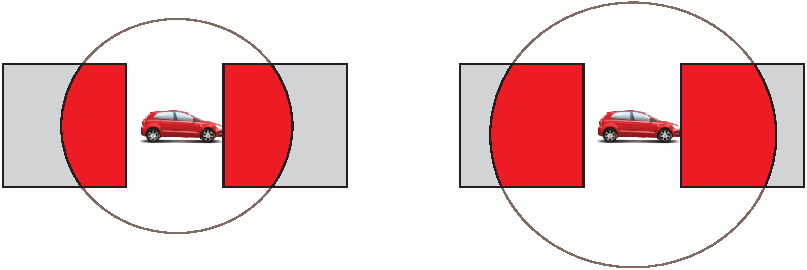
\includegraphics[scale=0.5]{resultados/figuras/problemaDisperdicio.pdf}
		\caption{Exemplificação do disperdicio.}
		\label{fig:problemaDisperdicio}
	\end{figure}


A princípio, não é necessário se preocupar com a economia de energia do transmissor/receptor instalado em cada veículo. Assim, o alcance da comunicação dos nós pode ser alta, melhorando o desempenho do agente. 

Quanto maior é a quantidade de veículos (nós) que formam a rede, maior é a probabilidade do agente alcançar novos nós hospedeiros, e assim maiores são as chances dele conseguir se manter na região alvo. A melhora de desempenho do agente comparando entre a situação onde o agente tem a disposição o menor alcance e a menor densidade de veículos (25 nós e 10 metros) para a situação mais farta de recursos (100 nós e 30 metros) é de 145\% aproximadamente.   


\subsubsection{Rede com infraestrutura}

	Os resultados obtidos em uma rede veicular com infraestrutura demonstrou que a densidade e raio de alcance tem os mesmos impactos discutidos na Seção \ref{subsubsection:redeSemInfraestruturaResultadoDiscucao}.

	Na Figura \ref{fig:graficosComTorres} demonstra a melhoria de desempenho do agente ao aumentar a densidade dos nós e o raio de alcance. A melhoria de desempenho do agente na configuração com a menor quantidade de recursos para a rede com a configuração com maior quantidade de recursos foi de 114,43\%.   
 

	\begin{figure}[htbp]
		\centering
		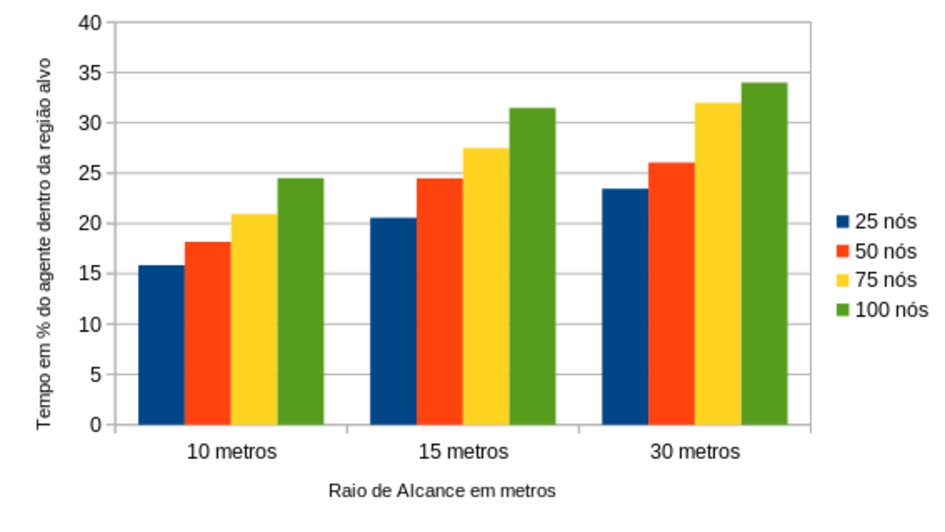
\includegraphics[scale=0.5]{resultados/graficos/graficoComTorres.pdf}
		\caption{Resultados obtidos no cenários com infraestrutura.}
		\label{fig:graficosComTorres}
	\end{figure}

	Para cada vinte e cinco nós que entram na rede, o agente melhora o seu desempenho (tempo médio dentro da região alvo) significativamente. O aumento do raio de alcance de cada nó também aumenta o desempenho do agente. O aumento combinado do raio e a densidade causa um impacto diretamente na quantidade de veículos que o agente tem acesso, aumentando o seu desempenho.

	Na Tabela \ref{tab:estatiscaResultadosObtidosComInfraestrutura} é possível visualizar a média aritmética, o desvio padrão e a variância dos resultados obtidos.

	\begin{table}[!htb]
	    \caption{Estatística dos resultados obtidos}
	    \label{tab:estatiscaResultadosObtidosComInfraestrutura}
	    \centering
	    \scriptsize
	    \begin{minipage}{.5\linewidth}
	      
	      \centering
	        \begin{tabular}{|c|c|c|}

			\hline
			\multicolumn{3}{|c|}{25 nós} \\ \hline
			Alcance   & média aritmética &	Desvio Padrão   \\ \hline
			10 metros &	15,85 & 1,40   \\ \hline
			15 metros &	20,57 & 1,68   \\ \hline
			30 metros &	23,45 & 1,11  \\ \hline

			\multicolumn{3}{|c|}{} \\ \hline

			\multicolumn{3}{|c|}{50 nós} \\ \hline
			Alcance   & média aritmética &	Desvio Padrão   \\ \hline
			10 metros &	18,18 & 1,43   \\ \hline
			15 metros &	24,48 & 1,12  \\ \hline
			30 metros &	26,05 & 1,41  \\ \hline

		\end{tabular}
	    \end{minipage}%
	    \begin{minipage}{.5\linewidth}
	      \centering
	        \begin{tabular}{|c|c|c|}
	        \hline
			\multicolumn{3}{|c|}{75 nós} \\ \hline
			Alcance   & média aritmética &	Desvio Padrão   \\ \hline
			10 metros &	20,94 & 2,05   \\ \hline
			15 metros &	27,50 & 1,69   \\ \hline
			30 metros &	31,99 & 1,38 \\ \hline

			\multicolumn{3}{|c|}{} \\ \hline


			\multicolumn{3}{|c|}{100 nós} \\ \hline
			Alcance   & média aritmética &	Desvio Padrão   \\ \hline
			10 metros &	24,51 & 1,10   \\ \hline
			15 metros &	31,49 & 1,13   \\ \hline
			30 metros &	34,00 & 1,42  \\ \hline

		\end{tabular}

	    \end{minipage} 
	\end{table} 

\subsection{Resultados com Protótipo}

Como descrito na Seção \ref{subsec:prototipoExperimento} foram realizados dois testes com o protótipo, o primeiro utilizando uma infraestrutura fixa e outro só com os veículos.

A Figura demonstra a comparação entre as médias das latências, pode-se observar que a infraestrutura não causou nenhum impacto na latência. Isso ocorre pelo fato que ambos os experimentos utilizaram os mesmos algoritmos de locomoção do agente e equipamentos. Levando em consideração que o ambiente era controlado e não existiam outras fontes de ruído, o Zigbee apresentou uma baixa variação da latência. A Tabela \ref{tab:experimentoRealLatencia} apresenta informações como média e variância.


\begin{figure}[htbp]
	\centering
	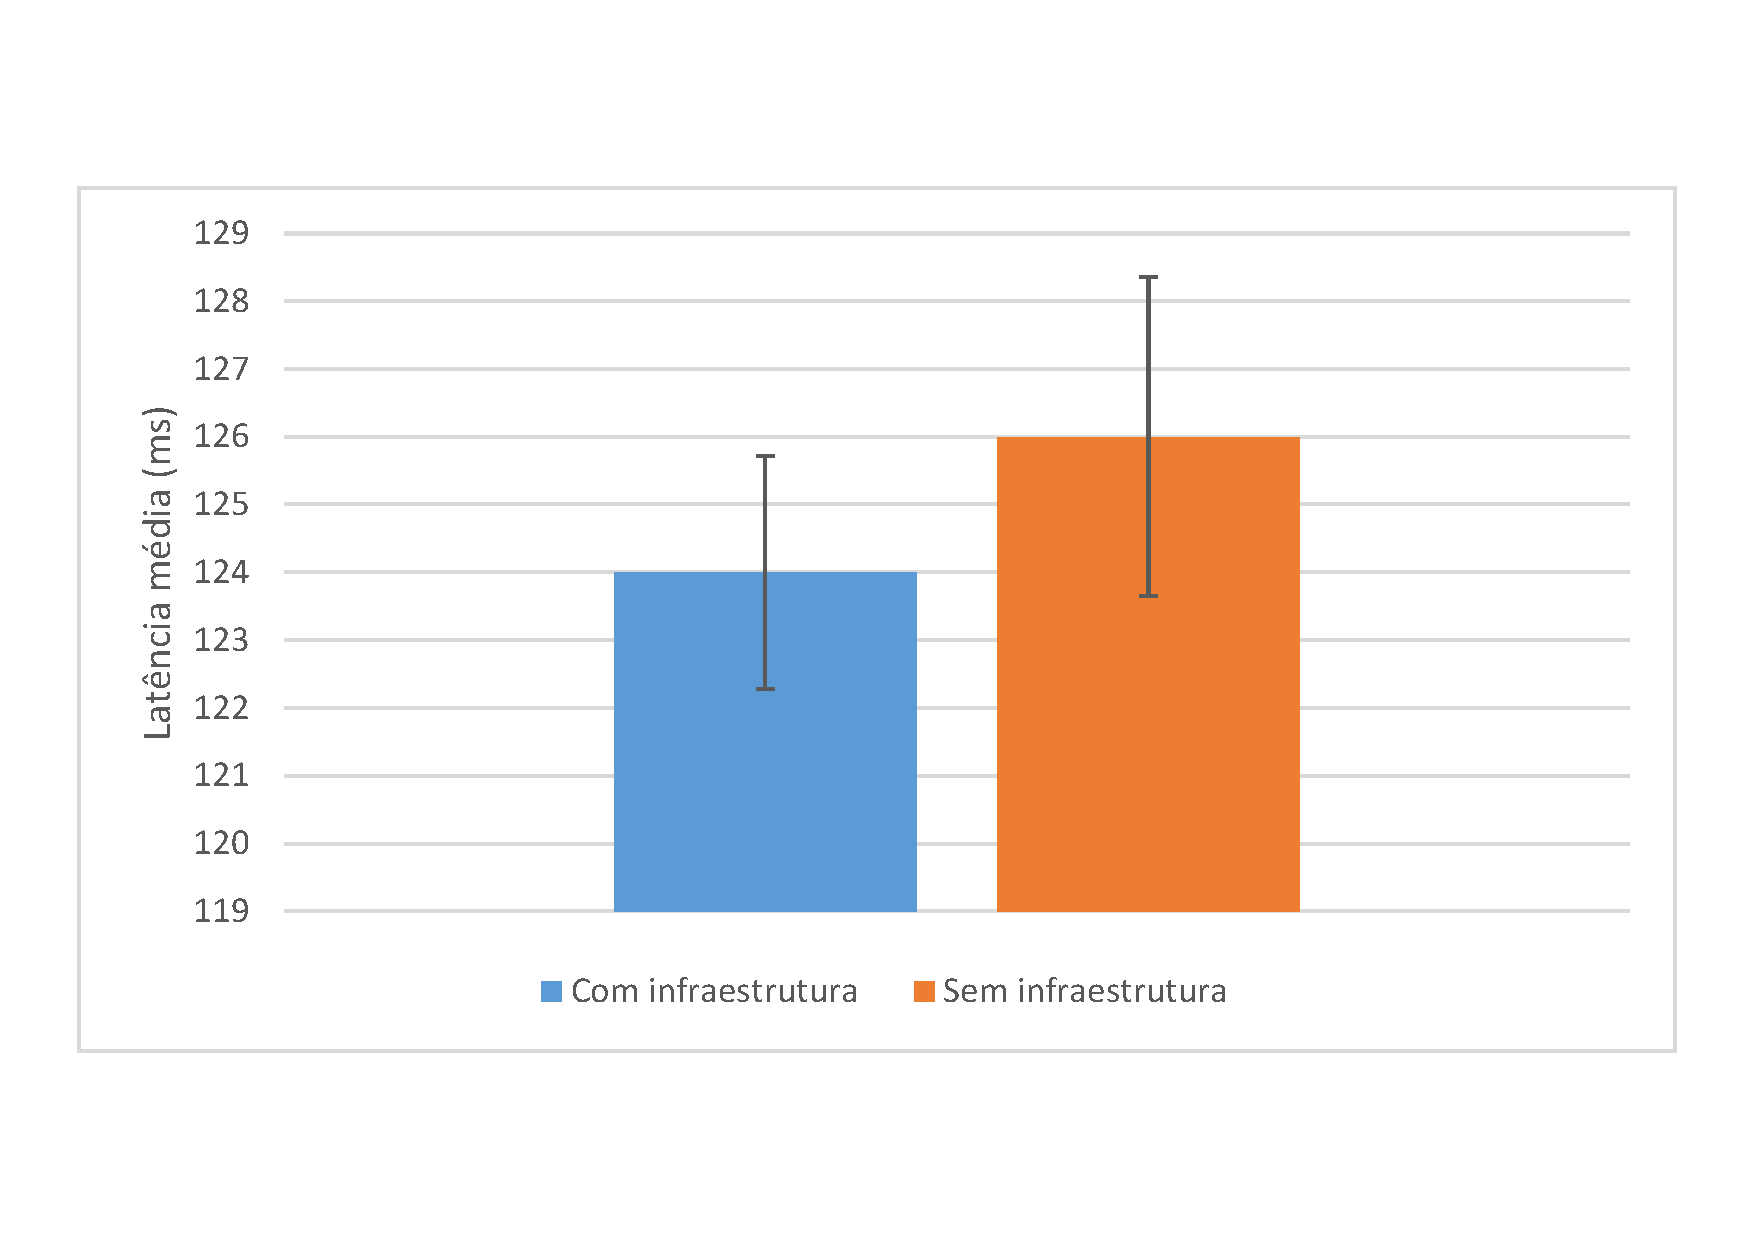
\includegraphics[scale=0.4]{resultados/graficos/experimentoRealLatencia.pdf}
	\caption{Latência obtida no experimento com o protótipo.}
	\label{fig:experimentoRealLatencia}
\end{figure}


\begin{table}[ht]
	\caption{Dados estatisticos da latência.}
	\centering
	\begin{tabular}{ | l | c | c | c|}
		\hline
		& média aritmetica & Desvio Padrão & Variância \\ \hline
		Sem infraestrutura & 126 (ms) & 2,3123 & 5,6288  \\ \hline
		Com infraestrutura & 124 (ms) & 1,7654 & 2,8354 \\ \hline
	\end{tabular}
	\label{tab:experimentoRealLatencia}
\end{table}

Com infraestrutura o agente realizou duzentos e setenta migrações e em vinte e nove o agente foi perdido. Quando é observado as migrações na situação sem infraestrutura o agente realizou duzentos e onze migrações e se perdeu em vinte e três migrações. A Tabela \ref{tab:migracoesPerda} demonstra o resultado da simulação em relação a migração e perda do agente.

\begin{table}[ht]
	\caption{Relação quantidade migração e perda.}
	\centering
	\begin{tabular}{ | l | c | c | c |}
		\hline
					& Migrações & Perda do agente & \% \\ \hline
		Sem infraestrutura & 211 & 45 & 21,32\%  \\ \hline
		Com infraestrutura & 270 & 23 & 10,74\%  \\ \hline
	\end{tabular}
	\label{tab:migracoesPerda}
\end{table}

O agente realiza mais migrações na situação com infraestrutura por que ela possui um nó a mais. Outro ponto importante é a porcentagem da taxa de perda do agente  em relação a quantidade de migração. Como a infraestrutura permanece estática, a velocidade relativa entre o nó no veículo e o nó da infraestrutura é a velocidade do veículo. Então o tempo que o agente tem para migrar e maior por que aumenta o tempo de comunicação entre os nós. No caso do experimento só com veículos a velocidade relativa é a soma das velocidades dos dois veículos, isso diminui o tempo que o agente tem para migrar, causando o aumento da perda do agente. As Figuras \ref{fig:velocidadeRelativaNegativa}, \ref{fig:velocidadeRelativaPositiva} e \ref{fig:velocidadeRelativaNeutra} exemplificam a velocidade relativa.


\begin{figure}[htbp]
	\centering
	\begin{minipage}{0.46\textwidth}
		\centering
		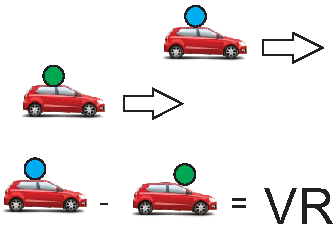
\includegraphics[scale=0.5]{resultados/figuras/velocidadeRelativaNegativa.pdf}
		\captionof{figure}{VR negativa.}
		\label{fig:velocidadeRelativaNegativa}
	\end{minipage}
	\begin{minipage}{0.46\textwidth}
		\centering
		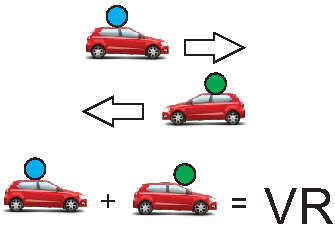
\includegraphics[scale=0.5]{resultados/figuras/velocidadeRelativaPositiva.pdf}
		\captionof{figure}{VR positiva.}
		\label{fig:velocidadeRelativaPositiva}
	\end{minipage}
	\begin{minipage}{0.46\textwidth}
		\centering
		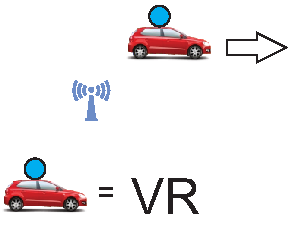
\includegraphics[scale=0.5]{resultados/figuras/velocidadeRelativaNeutra.pdf}
		\captionof{figure}{VR neutra.}
		\label{fig:velocidadeRelativaNeutra}
	\end{minipage}
\end{figure} 

%\include{cronograma}
%\section{Conclusão}

A área de redes veiculares tem um potencial muito amplo para realização de pesquisas.  As redes veiculares em sua configuração híbrida, até o momento, não foram totalmente exploradas e podem ser aprimoradas.

Os agentes móveis adicionam às redes veiculares maior flexibilidade para trafegar dados. Através do agente os dados podem ser transportados levando em consideração o contexto, assim o agente decide se deve ou não migrar para outro nó. Outro ponto importante é que o agente pode decidir, dependendo do contexto, em usar outras formas de comunicação. 

Nas simulações realizadas neste trabalho é possivel observar que a rede com infraestrutura melhora o desempenho do agente em comparação a uma rede sem infraestrutura. Porém, o impacto da infraestrutura em redes densas é menor. Essa informação é importante para auxiliar na escolha das regiões onde serão colocadas as infraestrturas. Regiões mais densas de veículos podem receber menos infraestruturas e regiões menos densas recebem mais infraestrutura. 

No experimento com o protótipo desenvolvido, o ZigBee se mostrou viável para transportar agente de software simples. Porém, os agentes possuem uma complexidade maior que as informações transportadas no trabalho \cite{santanaMestrado:2014} que obteve latência média de 64ms. No presente trabalho, a latência média foi de 124ms com infraestrutura e 126ms sem infraestrutura. Assim a latência se mostrou alta para aplicações críticas como, por exemplo, alerta de colisão entre veículos.

A taxa de perda do agente com infraestrutura foi de aproximadamente 10\% no experimentos com o protótipo, enquanto que sem infraestrutura foi obtido aproximadamente 21\% de perda. Essa informação mostra que o uso de infraestrutura como suporte na migração ajuda significativamente a diminuir a perda do agente.


\subsection{Proposta de continuidade}
Como proposta de continuidade para este trabalho, pode-se adicionar mais dispositivos de hardware ao protótipo para que o agente móvel possa extrair mais informações do ambiente para realizar a sua missão.

Outro trabalho a realizar é comparar o padrão ZigBee com o padrão 802.11p para transporte de agentes. Nesse trabalho é importante observar a latência e a perda do agente para comparar qual forma de comunicação é mais eficaz.

Desenvolver mecanismos mais eficientes para recuperar os agentes danificados durante a migração seria outra proposta de continuidade dos estudos para diminuir a taxa de perda do agente. 




%==============================================================================
% Incluindo bibliografia
%\bibliographystyle{plain}             % estilo para labels em numeros
%\bibliographystyle{alpha}             % estilo para labels em iniciais
% \bibliographystyle{abnt-alf}           % estilo para referências usando
%ABNT, 
% %\bibliographystyle{apalike}
% %\bibliographystyle{acm}
% %\bibliographystyle{plain}
% precisa instalar o abntex para usar!!!
%\bibliographystyle{abnt-alf}
%\addcontentsline{toc}{section}{REFER�NCIAS}
%{\def\section*#1{}
 %\renewcommand{\refname}{}
 %\begin{center}{\normalsize\bfseries REFER�NCIAS}\end{center}
%\bibliography{refbib}
%}
%inclui Referências Bibliográficas
\bibliography{refbib}			% arquivo exemplo refbib.bib

%\nocite{*}
%==============================================================================
% Incluindo anexos numerados com letras maiusculas.
%\appendix
%\include{apendice}

%==============================================================================
% Fim do texto
\end{document}
